% Twoside implica che i capitoli inizino sempre con la prima pagina a sinistra, eventualmente lasciando una pagina vuota nel capitolo precedente. 
\documentclass[a4paper, twoside,openright]{report}

%spazio interlinea
\usepackage{setspace}
\onehalfspacing
% Dimensione dei margini
\usepackage[a4paper,top=3cm,bottom=3cm,left=3cm,right=3cm]{geometry} 
% Dimensione del font
\usepackage[fontsize=13pt]{scrextend}
% Lingua del testo
\usepackage[english,italian]{babel}
% Lingua per la bibliografia
\usepackage[fixlanguage]{babelbib}
% Codifica del testo
\usepackage[utf8]{inputenc} 
% Encoding del testo
\usepackage[T1]{fontenc}
%font
\usepackage{helvet}

% Kerinig del testo
\usepackage[expansion=false]{microtype}
\SetTracking{encoding = *, shape = sc}{30}
% Per modificare l'header delle pagine 
\usepackage{fancyhdr}               

\usepackage{float}

% Librerie matematiche
\usepackage{amssymb}
\usepackage{amsmath}
\usepackage{amsthm}         

% Uso delle immagini
\usepackage{graphicx}
% Uso dei colori
\usepackage[dvipsnames]{xcolor}         
% Uso dei listing per il codice
\usepackage{listings} 
\lstset{
  backgroundcolor=\color{gray!10},   % colore dello sfondo
  basicstyle=\ttfamily,              % imposta il font del testo
  breaklines=true,                   % interrompi le linee troppo lunghe
  frame=single,                      % aggiungi una cornice intorno al codice
  captionpos=b,                      % posiziona la didascalia in basso
  numbers=left,                      % mostra i numeri di linea a sinistra
  numberstyle=\small,                % imposta lo stile del numero di linea
  showstringspaces=false,            % non mostrare gli spazi nelle stringhe come underscore
  escapeinside={(*@}{@*)},           % se vuoi inserire LaTeX all'interno del tuo codice
}
         
% Per inserire gli hyperlinks tra i vari elementi del testo 
\usepackage{hyperref}     
% Diversi tipi di sottolineature
\usepackage[normalem]{ulem}

% -----------------------------------------------------------------

% Modifica lo stile dell'header
\pagestyle{fancy}
\fancyhf{}
\lhead{\rightmark}
\rhead{\textbf{\thepage}}
\fancyfoot{}
\setlength{\headheight}{16pt}

% Rimuove il numero di pagina all'inizio dei capitoli
\fancypagestyle{plain}{
  \fancyfoot{}
  \fancyhead{}
  \renewcommand{\headrulewidth}{0pt}
}

\definecolor{backcolour}{rgb}{0.90,0.95,0.92}

% Stile del codice
% \lstset{style=codeStyle}
\lstdefinestyle{codeStyle}{
    backgroundcolor=\color{backcolour},
    commentstyle=\color{teal},
    keywordstyle=\color{Magenta},
    numberstyle=\tiny\color{gray},
    stringstyle=\color{violet},
    basicstyle=\ttfamily\scriptsize,
    breakatwhitespace=false,     
    breaklines=true,                 
    captionpos=b,                    
    keepspaces=true,                 
    numbers=left,                    
    numbersep=5pt,                  
    showspaces=false,                
    showstringspaces=false,
    showtabs=false,
    tabsize=1
} \lstset{style=codeStyle}

% \lstset{style=longBlock}
\lstdefinestyle{longBlock}{
    commentstyle=\color{teal},
    keywordstyle=\color{Magenta},
    numberstyle=\tiny\color{gray},
    stringstyle=\color{violet},
    basicstyle=\ttfamily\scriptsize,
    breakatwhitespace=false,         
    breaklines=true,                 
    captionpos=b,                    
    keepspaces=true,                 
    numbers=left,                    
    numbersep=5pt,                  
    showspaces=false,                
    showstringspaces=false,
    showtabs=false,                  
    tabsize=2
} \lstset{style=codeStyle}

% Togliendo il commento al comando che segue, si inseriscono nella bibliografia anche le fonti presenti in Bibliography.bib ma non citati direttamente con il comando \cite
\nocite{*}

% Margini prima e dopo blocchi di codice, per avere più distanza
\lstset{aboveskip=20pt,belowskip=20pt}

% Modifica dello stile dei riferimenti
\hypersetup{
    colorlinks,
    linkcolor=black,
    citecolor=black
}

% Aggiunti definizioni, teoremi, linea e listing
\newtheorem{definition}{Definizione}[section]
\newtheorem{theorem}{Teorema}[section]
\providecommand*\definitionautorefname{Definizione}
\providecommand*\theoremautorefname{Teorema}
\providecommand*{\listingautorefname}{Listing}
\providecommand*\lstnumberautorefname{Linea}

\raggedbottom



% -----------------------------------------------------------------
\begin{document}
\begin{titlepage}
\begin{figure}[!htb]
    \centering
\end{figure}
\vspace{30mm}
\begin{center}
    \LARGE{UNIVERSITÀ DEGLI STUDI DI MODENA E REGGIO EMILIA}
    \vspace{5mm}
    \\ \large{DIPARTIMENTO DI INGEGNERIA "ENZO FERRARI"}
    \vspace{5mm}
    \\ Laurea Triennale in Ingegneria Informatica
\end{center}

\vspace{15mm}
\begin{center}
    {\LARGE{\bf Planning locale\\ \vspace{5mm} di una vettura da Formula Student\\ \vspace{5mm} a guida autonoma}}
    
    % Se il titolo è abbastanza corto da stare su una riga, si può usare
    
    % {\LARGE{\bf Un fantastico titolo per la mia tesi!}}
\end{center}
\vspace{30mm}

\begin{minipage}[t]{0.47\textwidth}
	{\large{Relatore:}{\normalsize\vspace{3mm}
	\bf\\ \large{Prof: Francesco Guerra}}}
\end{minipage}
\hfill
\begin{minipage}[t]{0.47\textwidth}\raggedleft
	{\large{Candidato:}{\normalsize\vspace{3mm} \bf\\ \large{Filippo Gibertini}}}
\end{minipage}

\vspace{30mm}
\hrulefill
\\\centering{\large{Anno Accademico 2022/2023}}

\end{titlepage}
\let\cleardoublepage\clearpage
\include{chapters/Abstract}
\let\cleardoublepage\clearpage

\tableofcontents

\listoffigures

\chapter{introduzione}
Nell'ambito della guida autonoma il Planning è una componente software che si occupa di delineare la traiettoria che la macchina deve seguire. In particolare, nelle auto a guida autonoma da competizione, il Planning si suddivide in Locale e Globale. Il Planning Globale è specializzato nel navigare attraverso percorsi conosciuti, mentre il Planning Locale si occupa di generare la traiettoria della macchina attraverso percorsi di cui non si posseggono informazioni pregresse. Gli aspetti cruciali di cui si è dovuto tenere conto nella realizzazione dell'algoritmo di Planning Locale sono: \textit{(1)} la molteplicità delle prove di gara che si devono affrontare, ognuna delle quali necessita di un Planning Locale dedicato, \textit{(2)} la corretta comunicazione con gli altri elementi software (nodi) che compongono l'algoritmo di guida autonoma, \textit{(3)} la necessità di un algoritmo che si avvicini il più possibile ad essere real-time.

\chapter{Stato dell'arte}

arte dello stato
\chapter{Conoscenze di base} 
In questo capitolo verranno esplorate le conoscenze fondamentali che costituiscono il punto di partenza teorico per lo sviluppo del progetto. Queste conoscenze sono
 essenziali per comprendere appieno il contesto e i concetti chiave che saranno discussi
 nei prossimi capitoli.
 
\section{ROS2 - Robotic Operating System}
ROS2 è un middleware basato su un meccanismo di publisher e subscriber che per
mette l’interazione, attraverso lo scambio di informazioni, tra diversi processi ROS.\\
Il progetto è stato sviluppato all'interno di un workframe ROS2 (ROS Foxy)\cite{doi:10.1126/scirobotics.abm6074} instroduciamo quindi alcuni componenti della sua terminologia fondamentale \cite{rosDocumentation}: \\
\begin{enumerate}
\item \textbf{ROS graph}: Si riferisce ad una rappresentazione visuale o concettuale della rete
 di comunicazione e delle interconnesioni tra i nodi all’interno di ROS. Questa
 rappresentazione grafica mostra come i nodi comunicano tra loro, inviando e
 ricevendo messaggi tramite i topic e come sono collegati all’interno di ROS.
\item \textbf{ROS topic}: I topic vengono utilizzati come canali di comunicazione tra diversi processi, in modo da scambiarsi dati attraverso dei messaggi.
\item \textbf{ROS nodes}:  I nodi possono essere visualizzati come unità di elaborazione,
 ovvero sono quelle entità che si devono scambiare dati fra di loro, questo avviene tramite i publisher o subscriber, infatti i nodi hanno la capacità di:\\
 
\begin{itemize}

\item \textbf{Sottoscriversi} ad un topic e quindi rimanere in ascolto su di esso e ricevere tutti i messaggi che vengono pubblicati in quel determinato topic. Un comportamento di questo tipo è quello dei subscriber.
\item \textbf{Pubblicare}  messaggi su un certo topic e quindi invocare una chiamata di funzione per mandare un certo messaggio sul topic selezionato che poi verrà letto da tutti quei nodi che hanno un componente che si è sottoscritto a quel topic. Questi sono i publisher.

\begin{figure}[ht]
\centering
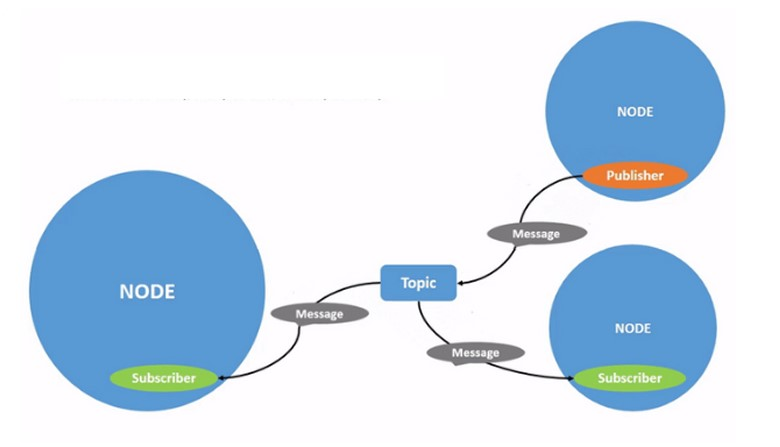
\includegraphics[width=\linewidth]{"images/nodi.jpg"}
\caption{Funzionamento protocollo pub/sub su ROS}
\label{fig:myImageLabel}
\end{figure}
\end{itemize}

\item \textbf{ROS message}:  I messaggi utilizzati in ROS sono strutture dati organizzate in campi, e per ciascun campo è specificato il tipo di dato che contiene. È possibile personalizzare i messaggi creando un file in cui si definiscono i campi necessari e salvandoli nel formato msg. ROS offre la possibilità non solo di definire nuovi tipi di messaggi, ma include anche una vasta libreria di messaggi predefiniti sviluppati dagli stessi creatori di  ROS, che coprono una vasta gamma di scenari. Questi tipi di messaggi personalizzati possono essere utilizzati non solo all’interno del nodo in cui sono stati definiti, ma anche in tutti i nodi in cui sono installate le dipendenze del nodo che utilizza quel messaggio.\\

\begin{figure}[t!]
\centering
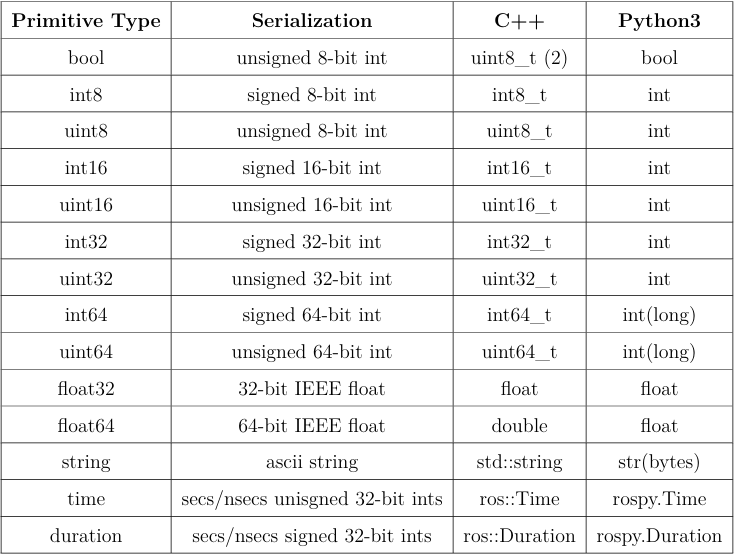
\includegraphics[width=\linewidth]{"images/tipi.png"}
\caption{Rappresentazione dei vari tipi su ROS}
\label{fig:myImageLabel}
\end{figure}
\end{enumerate}

Dopo aver introdotto la terminologia necessaria per riuscire a discutere di ROS
 in maniera appropriata, prendiamo in considerazione un nodo e andiamo a studiarne i
 componenti a livello implementativo.
\begin{lstlisting}[language=bash, caption={Creazione di un nodo ROS}]
$ source /opt/ros/foxy/setup.bash
$ ros2 pkg create -build-type ament_cmake <package_name>
\end{lstlisting}

Per ogni nodo sono presenti quattro directory principali oltre alla \textit{CMakeLists.txt} che rende la compilazione più snella da parte dell’utente e al \textit{package.xml} che definisce il pacchetto.
\begin{enumerate}
\item \textbf{config}: É presente un file di configurazione in cui possono essere definiti dei
 parametri statici che vengono poi recuperati dal nodo e utilizzati durante l’esecuzione. La comodità di utilizzare dei parametri di questo tipo è che non bisogna ricompilare il nodo se vengono modificati.
 
\begin{lstlisting}[language=bash, caption={Esempio di un file config}]
/package_name:
 	ros__parameters:
 	esempio_parametro: 1
 	general:
 	esempio_parametro: "prova"
\end{lstlisting}

\item \textbf{include/name\_node}: Si possono trovare tutti i file di intestazione che defini
scono le interfacce o le dichiarazioni delle classi, delle funzioni o delle variabili
 utilizzate all’interno del pacchetto. Questi file possono essere inclusi in altri file
 sorgente all’interno del pacchetto o in pacchetti esterni che desiderano utilizzare
 le funzionalità fornite dal pacchetto.
 
\item \textbf{launch}:  contengono i file che permettono al nodo di essere eseguito in maniera
 più snella e controllata. Per ogni file config che viene creato all’interno di un
 nodo è necessario aggiungere il percorso della directory in cui è presente il file di
 configurazione.
 
\begin{lstlisting}[language=bash, caption={Esempio di un file launch}]
def generate_launch_description() :
 	config_node = os.path.join
 	(
 	get_package_share_directory('package_name'),
'config',
'package_name_conf.yaml'

\end{lstlisting}
 \item \textbf{src}: Contiene il codice sorgente effettivo del pacchetto, inclusi i file sorgente per
 i nodi ROS2, le librerie personalizzate le classi e le funzioni che costituiscono il
 comportamento del pacchetto.
 
\end{enumerate}

L’ultima parte sulla visione iniziale di ROS2 è quella che riguarda la compilazione e
 l’installazione dei nodi all’interno del \textbf{ROS Environment}.
 
\begin{lstlisting}[language=bash, caption={ Compilazione di un pacchetto ROS e attivazione dell’Environment
}]
	$ colcon build --symlink-install
 --continue-on-error --package-select <package_name>
 
 # in questo modo posso eseguire file launch come se fossero nella cartella corrente
	$ source ./ros2_env/install/setup.bash
	$ ros2 launch package_name package_name_launch.py
\end{lstlisting}


\chapter{Implementazione}
In questo capitolo verrà descritto come è sono stati tradotti in codice gli algoritmi descritti nei capitoli precedenti.
E' stato implementato un planner per ogni prova della gara: \index{1}acceleration, \index{2}skidpad, \index{3}autocross e trackdrive, che condividendo lo stesso tracciato condividono lo stesso planner. 
Ogni planner viene inizializzato all'interno di un nodo ROS che ha anche le responsabilità di reperire il tipo della prova e istanziare  publishers e subscribers.
\section{Local planner node}
Il nodo è stato definito nel file \texttt{local\_planner\_node.h} ed è stato implementato nel file \texttt{local\_planner\_node.cpp}. Il nodo si prende a carico le seguenti responsabilità:
\begin{itemize}
	\item Reperire i parametri relativi ai topic e il parametro relativo al tipo di evento dal file di configurazione.
	\item Inizializzare i publishers che sono comuni a tutte le prove.
	\item Inizializzare il planner corrispondente al tipo di evento contenuto nel parametro "node/eventType". 
	\item inizializzare i subscribers specifici facendo il bind fra le callback del planner e i topic necessari.
\end{itemize} 
\include{chapters/project}
\chapter{Conclusioni}

L'applicazione, descritta all'interno di questa elaborato, ovviamente non è ultimata ma è solamente un punto di partenza per l'introduzione della programmazione modulare all'interno della libreria WLDT.   Difatti il progetto può essere, sicuramente,  migliorato ed ampliato sviluppando diverse tipologie di DigitalAdapter e PhysicalAdapter “complessi” (HTTPDigitalAdapter e MQTTPhysicalAdapter). Inoltre la flessibilità e la dinamicità tra le varie componenti del Digital Twin può essere, ulteriormente, migliorata riducendo la dipendenza tra il bundle rappresentante il modello del DT ed il bundle della ShadowingFunction, permettendo al Digital Twin di utilizzare più ShadowingFunction senza resettare lo stato interno. Infine potrebbe essere sviluppato anche un ulteriore bundle, che attraverso l'utilizzo di un event bus, gestisca la comunicazione tra i vari componenti del Digital Twin.
\bibliographystyle{unsrt}
\bibliography{main}
\end{document}